\documentclass{article}

\usepackage[a4paper, total={6in, 9in}]{geometry}

\usepackage{amsmath} % For math
\usepackage{amssymb} % For math
\usepackage{amsthm} % For math
\usepackage{esint} % For math
\usepackage{siunitx} % For SI units

\usepackage{graphicx} % For figures
\usepackage{subcaption} % For figure

\usepackage{float} % For figure placement

\usepackage{minted} % For code

\usepackage{hyperref} % For links
\hypersetup{
	colorlinks,
	citecolor=black,
	filecolor=black,
	linkcolor=black,
	urlcolor=blue,
}
\usepackage{cleveref} % For references

\usepackage{parskip} % For paragraph spacing and no indentation

% \usepackage{tabularx} % For tables
\usepackage[table,xcdraw]{xcolor} % For tables
\def\arraystretch{1.5} % Better looking tables
\usepackage{adjustbox}

% Costum commands:

\newcommand{\qr}{{\quad\Rightarrow\quad}}
\newcommand{\qqr}{{\qquad\Rightarrow\qquad}}



\title{Exam Numerical Methods 2025}
\author{Mathias Balling}
\date{\today}

\begin{document}
\maketitle

Code used for the exercises can be found in "exam/", "utils/", and "Numerical-Recipes/".
\section*{Exercise 1}
\subsection*{i}
Using method of SVD from NR3 headers.
\begin{minted}{cpp}
SVD svd_solver(A);
util::print(svd_solver.w, "w");
\end{minted}

\texttt{w} is as follows:\\
$11.951932409770585$\\
$5.397266515466196$\\
$4.719596639028403$\\
$3.953906595603368$\\
$3.6230909930002446$\\
$3.368300112475192$\\
$3.0916664682435697$\\
$4.811863543913732\cdot 10^{-15}$

\subsection*{ii}
Using method of SVD from NR3 headers.
\begin{minted}{cpp}
double threshold = 1e-14;
SVD svd_solver(A);
auto nullspace = svd_solver.nullspace(threshold);
util::print(nullspace, "nullspace");
\end{minted}
This could also be done by finding the index of the 0 element in w and then taking the corresponding column of V.

The unit vector in the null space of A is:\\
$0.30414953233623704$\\
$-0.6995439243733448 $\\
$6.934350372534523\cdot 10^{-17}$\\
  $-7.275658594236239\cdot 10^{-17}$\\
$0.42580934527073205$\\
$-3.3958678618647428\cdot 10^{-18}$\\
  $3.11158887096989\cdot 10^{-17}$\\
$-0.4866392517379791$\\

\subsection*{iii}
Using the SVD solver from NR3 headers.
\begin{minted}{cpp}
double threshold = 1e-14;
SVD svd_solver(A);
VecDoub x_sol(A_width);
svd_solver.solve(b, x_sol, threshold);
util::print(x_sol, "x_sol");
\end{minted}

\texttt{x} is as follows:\\
$-47.248363616439306$\\
$0.3688425226349671$\\
$79.65376424734224$\\
$-4.71197096346749$\\
$40.40427152514301$\\
$69.74266521165164$\\
$-42.73505350336738$\\
$5.29329919793784$

\subsection*{iv}
Code for linear regression error calculations can be found in "utils/linreg\_error.h"

The residual error of $5.42797258495411\cdot 10^{-6}$ is considarably smaller compared to the random fitting of $0.9128709291752769$, which a good starting point for accuracy validation.

The std. dev. of the estimated parameters:\\
$0.08468563169399769$\\
$0.16099885651146362$\\
$0.27703518823386664$\\
$0.2750301024010811$\\
$0.22661912057496514$\\
$0.2597660651878672$\\
$0.2503745120251377$\\
$0.22830996340629964$

The std. dev. of the estimated parameters are relativly small indicating the results have approced the correct values.
The std. dev. of the estimated parameters are calculated as follows using \texttt{V} and \texttt{w} from the SVD solver:
\begin{minted}{cpp}
VecDoub calculate_standard_deviation_svd(SVD &svd_solver, double threshold) {
  auto w = svd_solver.w;
  auto V = svd_solver.v;
  auto sigma = VecDoub(w.size());
  double sum;
  for (int j = 0; j < w.size(); j++) {
    sum = 0;
    for (int i = 0; i < w.size(); i++) {
      if (w[i] > threshold) {
        sum += pow(V[j][i] / w[i], 2);
      }
    }
    sigma[j] = sqrt(sum);
  }
  return sigma;
}
\end{minted}  

\newpage
\section*{Exercise 2}
\begin{minted}{cpp}
Vector function setup:
VecDoub vecfunc(VecDoub_I x) {
  assert(x.size() == 4);

  VecDoub f(4);

  f[0] = 3 * x[0] + x[1] * sin(x[2]) - cos(x[0]) + cos(pow(x[1], 2)) + 4.2;
  f[1] = 3 * x[1] + x[0] * x[2] * x[3] + sin(x[1]) - 5.1;
  f[2] = -pow(x[1], 2) + x[2] * pow(x[3], 2) + 3 * x[2] + 5.2;
  f[3] = x[0] + 3 * x[3] + sin(pow(x[2], 2) * pow(x[3], 2)) + cos(x[1]) - 2.3;
  return f;
}
\end{minted}

\subsection*{i}
When evaluating the function with $x_0=-0.7\quad x_1=1.2\quad x_2=2.3\quad x_3=-4.1$ the result is:\\
$2.3604277760657215$\\
$6.033039085967225$\\
$49.32299999999999$\\
$-14.118275390737853$


\subsection*{ii}
\begin{minted}{text}
| k  |       x_k      |        d_k       |      C     |       e        | lambda |
|----|--------------- |----------------- |----------- |----------------|--------|
| 1  |                |                  |            |                |  No BT |
|1(0)| -1.40000000851 |                  |            |                |        |
|1(1)|  1.27500000775 |                  |            |                |        |
|1(2)| -1.73333334387 |                  |            |                |        |
|1(3)| 0.899999998808 |                  |            |                |        |
| 2  |                |                  |            |                |  No BT |
|2(0)| -2.52981246183 |  -1.12981245332  |            |                |        |
|2(1)| 0.206707041083 |  -1.06829296667  |            |                |        |
|2(2)|  -1.6594756569 |  0.0738576869645 |            |                |        |
|2(3)| 0.892282003669 | -0.0077179951390 |            |                |        |
| 3  |                |                  | 0.10966935 | 0.007745490374 |0.111687|
|3(0)| -2.37494239018 |   0.15487007165  |            |                |        |
|3(1)| 0.382163475623 |   0.17545643454  |            |                |        |
|3(2)| -1.69981398652 | -0.0403383296173 |            |                |        |
|3(3)| 0.772996796054 |  -0.119285207615 |            |                |        |
| 4  |                |                  |  20.347090 | 42.0178871606  |  No BT |
|4(0)|  -1.2746127961 |   1.10032959407  |            |                |        |
|4(1)|  1.22281361303 |  0.840650137408  |            |                |        |
|4(2)| -1.36896314904 |  0.330850837483  |            |                |        |
|4(3)| 0.577609614918 |  -0.195387181136 |            |                |        |
| 5  |                |                  | 0.20976732 | 0.039362012827 |  No BT |
|5(0)| -0.97107267384 |  0.303540122259  |            |                |        |
|5(1)|  1.11854284125 |  -0.104270771779 |            |                |        |
|5(2)| -1.11800236852 |  0.250960780519  |            |                |        |
|5(3)| 0.724768551128 |  0.147158936209  |            |                |        |
| 6  |                |                  | 0.14970545 | 0.000118138606 |  No BT |
|6(0)| -0.96667857465 | 0.00439409918669 |            |                |        |
|6(1)|  1.13440513728 |  0.0158622960234 |            |                |        |
|6(2)| -1.10244628986 |  0.0155560786568 |            |                |        |
|6(3)| 0.741388663637 |  0.0166201125093 |            |                |        |
| 7  |                |                  | 0.59612044 | 1.31919941e-07 |  No BT |
|7(0)| -0.96634644910 | 0.00033212555338 |            |                |        |
|7(1)|  1.13461605039 | 0.00021091311314 |            |                |        |
|7(2)| -1.10221138134 | 0.00023490852128 |            |                |        |
|7(3)| 0.741495076632 | 0.00010641299509 |            |                |        |
\end{minted}

\subsection*{iii}
The accuracy is estimated as $e=1.31919941514e-07$ with the convergence constant $C=0.596120441159$

The error is calculated as follows ($d_k$ is a vector of the difference in x from last iteration to current iteration):
$$
C=\frac{||d_k||}{||d_{k-1}||^2}
$$
The convergence constant is then used to calculate the error:
$$C\cdot||d_k||^2$$

The code for error calculation is in "utils/multi\_roots.h"

\newpage
\section*{Exercise 3}

\subsection*{i}
The 2nd order system is:
$$
x''(t)=a_{max}\left(
  1-\left(\frac{x'(t)}{v_{des}}\right)^4
  -\left( \frac{D_0+\text{Max}\left(0,x'(t)T_{react}+\frac{x'(t)(x'(t)-X_F'(t))}{2a_{com}}\right)}{X_F(t)-x(t)} \right)^2
\right)
$$
From the 2nd order system we can make 2 1st order systems with new variables
$x_1(t)=x(t)$, $x_2(t)=x'(t)$:

$$
\begin{aligned}
  x_1'(t) &= x_2(t) \\
  x_2'(t) &=a_{max}\left(
    1-\left(\frac{x_2(t)}{v_{des}}\right)^4
    -\left( \frac{D_0+\text{Max}\left(0,x_2(t)T_{react}+\frac{x_2(t)(x_2(t)-X_F'(t))}{2a_{com}}\right)}{X_F(t)-x_1(t)} \right)^2\right)
\end{aligned}
$$

\subsection*{ii}
Setup of the ODE system:
\begin{minted}{cpp}
double a_max = 4.0;
double v_des = 25.0;
double D_0 = 50.0;
double T_react = 1.5;
double a_com = 2.0;

double X_F(double t) { return 250 + 15 * t - 5 * sqrt(1 + pow(t, 2)); }
double X_F_prime(double t) { return 15 - (5 * t) / sqrt(1 + pow(t, 2)); }

VecDoub derivs(const Doub t, VecDoub_I &x) {
  double x1 = x[0];
  double x2 = x[1];
  VecDoub_O dxdt(2);
  dxdt[0] = x2;
  dxdt[1] = a_max * (1 - pow((x2 / v_des), 4) - pow((D_0 + std::max(0.0, x2 * T_react +
              (x2 * (x2 - X_F_prime(t))) / (2 * a_com))) / (X_F(t) - x1), 2));
  return dxdt;
}
\end{minted}

The resulting value of the initial conditions with $t_0=-10$ is:\\
$x'(-10)=15.0$ and $x''(-10)=-1.2035371947583346$.

\subsection*{iii}
The plot can be seen here and is made using "exam/exam3\_plot.py":
\begin{figure}[H]
  \centering
  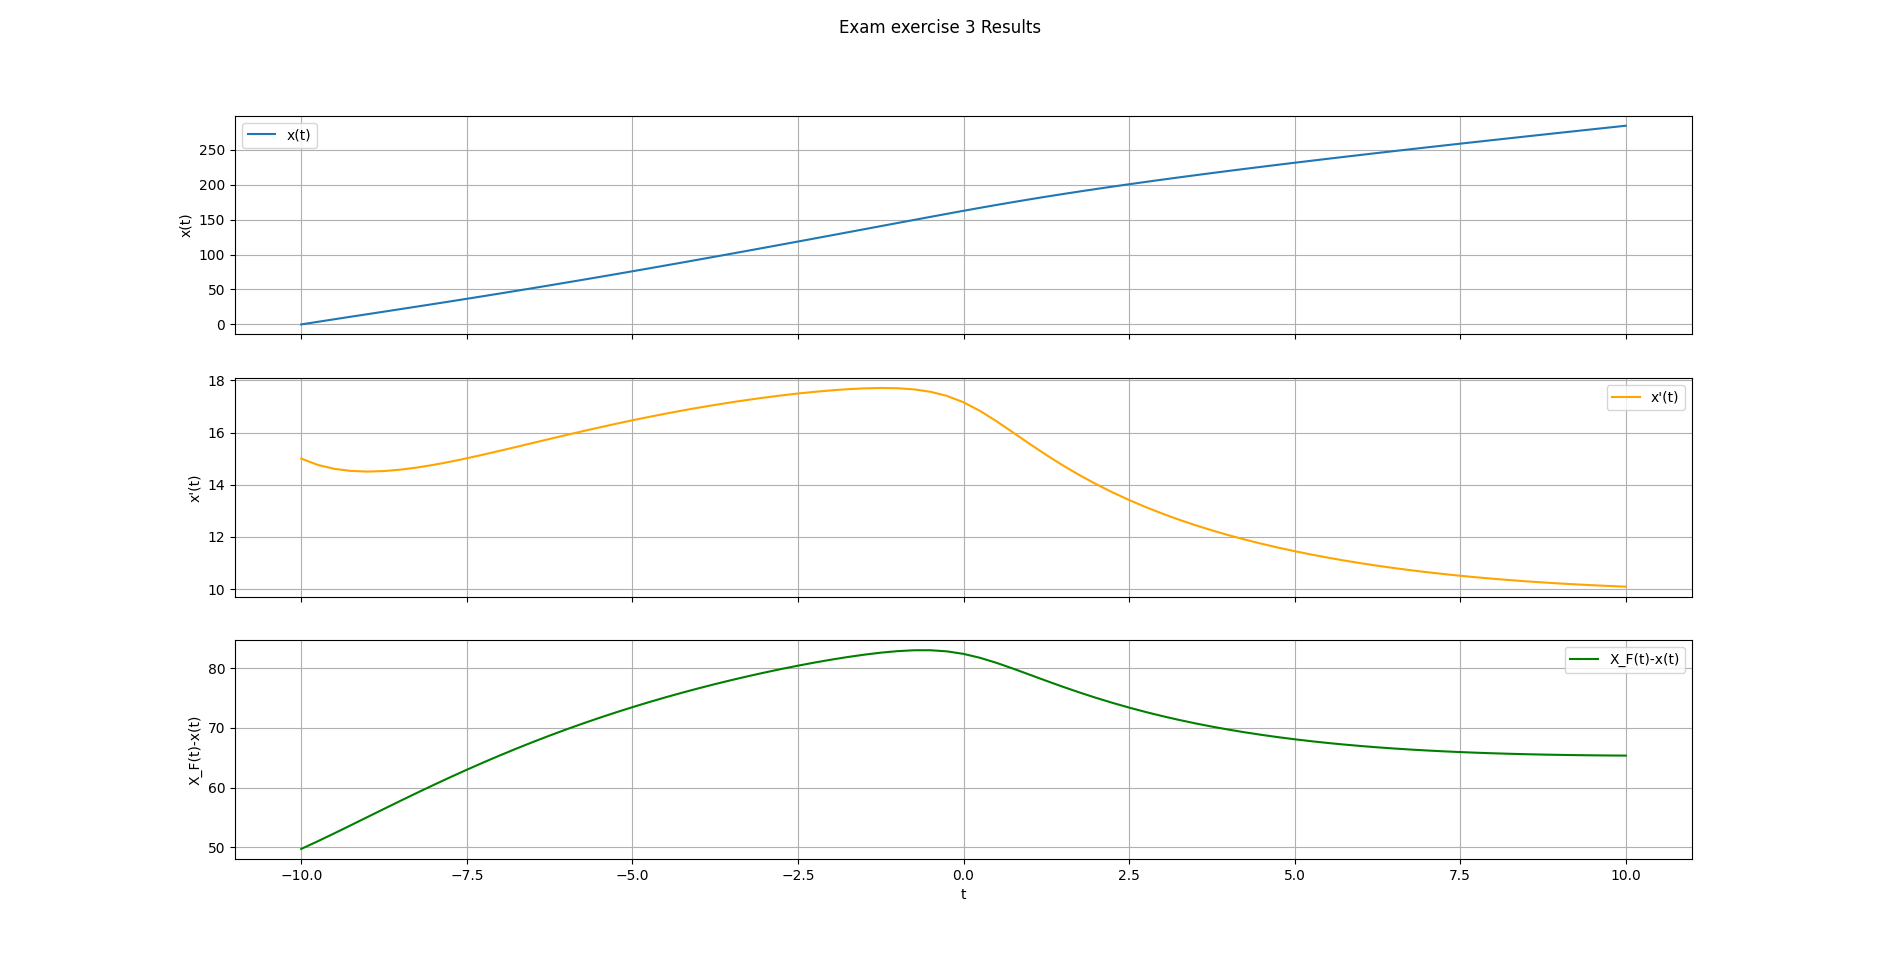
\includegraphics[width=\textwidth]{../exam3_plot.png}
\end{figure}

$x(10)=284.3842346596431$ and $x'(10)=10.092177928387363$

Code:
\begin{minted}{cpp}
// Midpoint method
VecDoub second_order_runge_kuttea_method_plot(double low, double high,
                                              int steps, VecDoub_I &x,
                                              VecDoub derivs(const Doub t,
                                                             VecDoub_I &x)) {
  std::vector<std::vector<double>> plotting;
  const double h = (high - low) / (double)steps;
  VecDoub x_n = x;
  plotting.push_back({low, x_n[0], x_n[1], (X_F(low) - x_n[0])});
  for (double t_n = low; t_n < high; t_n += h) {
    f_comps_current += 2;
    auto k1 = h * derivs(t_n, x_n);
    auto k2 = h * derivs(t_n + 0.5 * h, x_n + 0.5 * k1);
    auto x_n_next = x_n + k2;
    x_n = x_n_next;
    plotting.push_back({t_n + h, x_n[0], x_n[1], (X_F(t_n + h) - x_n[0])});
  }

  std::ofstream file;
  file.open("exam3_results.txt");
  for (const auto &vec : plotting) {
    std::println(file, "{}\t{}\t{}\t{}", vec[0], vec[1], vec[2], vec[3]);
  }
  file.close();

  return x_n;
}
\end{minted}
\subsection*{iv}
Based on the provided graph we see the car in front slows down from around 20 to around 10, which matches the plot from exercise iii vel. 
We both see the car slowing down and the distance between the car and the car in front is decreasing at around $t=0$ until the speeds match again.

\subsection*{v}
\begin{minted}{text}
For x(10)
|   N  |     A(N)    |   A(N/2)-A(N)  |alpha^k|    Rich error     |  Order est. |f comps|
|------|-------------|----------------|-------|-------------------|-------------|-------|
|  20  | 284.30333445|                |       |                   |             |   40  |
|  40  | 284.37167114| -0.06833668906 |       | 0.0227788963566   |             |   80  |
|  80  | 284.38423466| -0.01256351530 |5.43929| 0.00418783843344  | 2.443420160 |  160  |
|  160 | 284.38702585| -0.00279119785 |4.50111| 0.00093039928557  | 2.170283890 |  320  |
|  320 | 284.38768707| -0.00066122196 |4.22127| 0.000220407322293 | 2.077677835 |  640  |
|  640 | 284.38784818| -0.00016110802 |4.10421| 5.37026762875e-05 | 2.037106261 |  1280 |
| 1280 | 284.38788796| -3.9773799e-05 |4.05060| 1.3257933252e-05  | 2.018138092 |  2560 |
For x'(10)
|   N  |     A(N)    |   A(N/2)-A(N)  |alpha^k|    Rich error     |  Order est. |f comps|
|------|-------------|----------------|-------|-------------------|-------------|-------|
|  20  | 10.116751370|                |       |                   |             |   40  |
|  40  | 10.096355282|   0.02039608843|       | -0.00679869614505 |             |   80  |
|  80  | 10.092177928|  0.004177354050|4.88253| -0.00139245135016 | 2.2876311694|  160  |
|  160 | 10.091213181|  0.000964746857|4.33000| -0.00032158228567 | 2.1143670800|  320  |
|  320 | 10.090980755|  0.000232425688|4.15077| -7.7475229565e-05 | 2.0533809082|  640  |
|  640 | 10.090923676|  5.70791552e-05|4.07198| -1.9026385067e-05 | 2.0257336429|  1280 |
| 1280 | 10.090909531|  1.41453933e-05|4.03517| -4.7151311086e-06 | 2.0126316896|  2560 |
\end{minted}

From the table we can see that with $N=1280$ or $h=0,015625$ the estimated error for $x(10)$ is better than $2\cdot 10^{-5}$.
Error estimation is done using Richardson.

\newpage
\section*{Exercise 4}

Equation is set up as follows:
\begin{minted}{cpp}
double eqn(double x) { return exp(pow(x, 3)) * sqrt(x * (2 - x)); }
\end{minted}

\subsection*{i}
\begin{minted}{text}
| its   |  A(i)      |     A(i-1)-A(i)     | alpha^k  | Rich error    |  Order est.  |f comps|
|-------|------------|---------------------|--------- |---------------|------------- |-------|
|  2    |3.6243757712|                     |          |               |              |   3   |
|  4    |18.432965615|   -14.8085898439    |          | 0.98723932292 |              |   5   |
|  8    |54.698586304|   -36.2656206892    | 0.408336 | 2.41770804595 | -1.292168275 |   9   |
|  16   |86.718876557|   -32.0202902529    | 1.132582 | 2.13468601686 | 0.1796161555 |   17  |
|  32   |100.11196736|   -13.3930908053    | 2.390806 | 0.89287272035 | 1.2574974468 |   33  |
|  64   |104.35400456|   -4.24203720557    | 3.157230 | 0.28280248037 | 1.6586597591 |   65  |
| 128   |105.70663979|   -1.35263522555    | 3.136128 | 0.09017568170 | 1.6489844440 |  129  |
| 256   |106.15990895|   -0.453269157456   | 2.984176 | 0.03021794383 | 1.5773329282 |  257  |
| 512   |106.31622467|   -0.156315726242   | 2.899702 | 0.01042104841 |  1.535905068 |  513  |
| 1024  |106.37085226|  -0.0546275897805   | 2.861479 | 0.00364183931 | 1.5167612523 |  1025 |
| 2048  |106.39005897|  -0.0192067023301   | 2.844194 | 0.00128044682 | 1.5080199328 |  2049 |
| 4096  |106.39683117|  -0.00677220593843  | 2.836107 | 0.00045148039 | 1.5039120881 |  4097 |
| 8192  |106.39922231|  -0.00239113439314  | 2.832214 | 0.00015940895 | 1.5019306266 |  8193 |
|16384  |106.40006714| -0.000844831994243  | 2.830307 | 5.6322132e-05 | 1.5009588421 | 16385 |
|32768  |106.40036573| -0.000298594312255  | 2.829363 | 1.9906287e-05 | 1.5004777866 | 32769 |
|65536  |106.40047128| -0.000105551581555  | 2.828894 | 7.0367721e-06 | 1.5002384889 | 65537 |
|131072 |106.40050860| -3.73150385116e-05  | 2.828660 | 2.4876692e-06 | 1.5001191155 | 131073|
|262144 |106.40052179| -1.31923135172e-05  | 2.828543 | 8.7948756e-07 | 1.5000595849 | 262145|
|524288 |106.40052645| -4.66409086641e-06  | 2.828485 | 3.1093939e-07 | 1.5000297894 | 524289|
|1048576|106.40052810|  -1.6489892829e-06  | 2.828454 | 1.0993261e-07 | 1.5000138731 |1048577|
\end{minted}

\subsection*{ii}
First we find $alpha_k$:
$$
\frac{106.40052179-106.40052645}{106.40052645-106.40052810}=2.8245
$$
Then since we double each time we find order=$\log_2(alpha_k)$.
The order estimate is $\log_2(2.8245)=1.49786$. The same is shown in the table but with higher precision.
\subsection*{iii}
This is far from the expected order of 4. It could be a result of the singularities at the endpoints $x=0$ and $x=2$. Here we get $\sqrt{0}$ at both ends of the function which is not good.

\subsection*{iv}
The table shows Richardson extrapolation error using the expected order of 4. With the estimated order of around 1.5 the error will be:
$$
\frac{106.40052810-106.40052645}{(2.8245-1)}=9.04357\cdot10^{-7}
$$

This error is higher because of the lower computed alpha\_k estimate.

This is from the Richardson extrapolation error:
$$\frac{A(h_2)-A(h_1)}{alpha_k-1}$$

\subsection*{v}
Generally Simpson is better because of the higher expected order, where Midpoint and Trapezoid are both second order methods.

The midpoint methods is though expected to outperform the other two methods here since there is no function evaluating at the endpoints (singularities). This makes it more stable in this case.

\newpage
\section*{Exercise 5b}

\subsection*{i}
$$
\begin{aligned}
  \frac{\partial u(x,t)}{\partial t} &= 4\frac{\partial^2u(x,t)}{\partial x^2}+\sin{(\pi x)\exp{(-t)}}\\
  u(x,t)&=x^2\\
  u(0,t)&=0\\
  u(1,t)&=1+\sin{(t)}
\end{aligned}
$$
For $N=2$, $\alpha=4$, and $\Delta x=1/N=0.5$, the semidiscrete form using Euler is:
$$
\left\{
\begin{aligned}
  \frac{d u_j(t)}{dt}&=\frac{4}{0.5^2}(u_{j-1}(t)-2u_{j}(t)+u_{j+1}(t))+\sin(\pi x_j)\exp{(-t)}&j=1,\dots,2-1\\
  u_j(0)&=g(x_j) &j=0,\dots,2\\
  u_0(t)&=a(t)&t>0\\
  u_2(t)&=b(t)&t>0\\
\end{aligned}
\right.
$$
For the system:
$$\frac{du_1(t)}{dt}$$
at $t=0$ we have:
$$
\frac{d u_1(0)}{dt}=\frac{4}{0.5^2}(u_0(0)-2u_1(0)+u_2(0))+\sin(\pi 0.5)\exp{(-0)}
$$
and further reduced:
$$
\frac{d u_1(0)}{dt}=16(0-2\cdot 0.5^2+1)+1\cdot 1=9
$$

\subsection*{ii}
The parabolic PDE system is set up as follows:
\begin{minted}{cpp}
double u(double x, double t) {
  if (t == 0.0) {
    return pow(x, 2);
  }
  if (x == 0.0) {
    return 0.0;
  }
  if (x == 1.0) {
    return 1 + sin(t);
  }

  assert(false && "Not possible");
  return 0;
}

double f(double x, double t) { return sin(std::numbers::pi * x) * exp(-t); }

double alpha = 4.0;
double x_target = 0.5;
double t_target = 10.0;
\end{minted}

The code was not able to reach the accuracy of $10^{-7}$ after 10 hours of computation.
But it reached the accuracy of $10^{-6}$ after reasonable time, and that is used as shown in the table.

\begin{minted}{text}
|  N   |      A(N)      |    A(N/2)-A(N)   |    alpha^k  |  Rich error  |Order est.|  f comps   |
|------|--------------- |------------------|------------ |------------- |----------|------------|
|  4   | 0.096352855562 |                  |             |              |          |   246      |
|  8   | 0.107138879158 | -0.010786023595  |             | 0.0035953411 |          |   1134     |
|  16  | 0.113959604474 | -0.0068207253164 | 1.581360206 | 0.0022735751 | 0.661166 |   4830     |
|  32  |  0.11731649895 | -0.0033568944762 | 2.031855741 | 0.0011189648 | 1.022797 |  19902     |
|  64  | 0.118986866406 | -0.0016703674554 | 2.009674257 | 0.0005567891 | 1.006961 |  80766     |
| 128  | 0.119822117869 | -0.0008352514628 | 1.999837808 | 0.0002784171 | 0.999882 |  325374    |
| 256  | 0.120239761946 | -0.0004176440777 | 1.999912143 | 0.0001392146 | 0.999936 | 1306110    |
| 512  | 0.120448589975 | -0.0002088280283 | 1.999942636 | 6.960934e-05 | 0.999958 | 5233662    |
| 1024 | 0.120553005662 | -0.0001044156872 | 1.999967954 | 3.480522e-05 | 0.999976 | 20953086   |
| 2048 | 0.120605213943 | -5.220828085e-05 | 1.999983250 | 1.740276e-05 | 0.999987 | 83849214   |
| 4096 | 0.120631318182 | -2.610423899e-05 | 1.999992448 | 8.701412e-06 | 0.999994 |335470590   |
| 8192 | 0.120644370273 | -1.305209137e-05 | 2.000004308 | 4.350697e-06 | 1.000003 |1342029822  |
|16384 | 0.120650896099 | -6.525826005e-06 | 2.000067327 | 2.175275e-06 | 1.000048 |5368414206  |
|32768 | 0.120654158096 | -3.261996981e-06 | 2.000561632 | 1.087332e-06 | 1.000405 |21474246654 |
|65536 |  0.12065578548 | -1.627384007e-06 | 2.004442077 | 5.424613e-07 | 1.003200 |85898166270 |
|131072|  0.12065658454 | -7.990601963e-07 | 2.036622541 | 2.663533e-07 | 1.026178 |343595024382|
\end{minted}

The estimate for $u(0.5,10)$ is $0.12065658454$ at $N=131072$.

The error is calculated using Richardson extrapolation error using the expected order of 2 for the method. 
The estimated order is though only around 1 which could indicate bad convergence.

\end{document}
